\section{Dictionary Learning}
\label{sec:DictionaryLearning}

Sparse decomposition, just as the name implies, is a kind of matrix decomposition whose result matrices contain a simple matrix(e.g., transformation matrix\cite{le2012smooth}) and the correspondent coefficient matrix which is as sparse as possible. Generally this matrix decomposition is achieved with some iterative algorithm, so we could also class it into the learning based method just like the dictionary learning algorithm. The following works show its success in different applications.

\subsection{Skinning}

Skinning mesh animations has been an active area. Among many proposed techniques, $linear blending skinning$(LBS) is widely known to be the most popular skinning computational model due to its efficiency, simplicity, and effectiveness. In the LBS model, skin deformation is driven by a set of bones. Every vertex is associated with the bones via a bone-vertex weight map which quantifies the influence of each bone to the vertices. The skin is deformed by transforming each vertex through a weighted combination of bone transformations from the rest pose. By posing sparseness constraint on the weight map, the number of non-zero bone weights per vertex can be limited.

But the LBS model has certain limitations such as collapsing elbow and candy-wrapper effects and failure of secondary deformation. \cite{le2012smooth} introduces the Smooth Skinning Decomposition with Rigid Bones(SSDR), an automated algorithm to extract the linear blending skinning. The SSDR model can effectively approximate the skin deformation of nearly articulated models as well as highly deformable models by a low number of rigid bones and a sparse, convex bone-vertex weight map. The SSDR model is solved by a block coordinate descent-based algorithm to update the weight map and the bone transformations iteratively as mentioned above.

However, the sparseness constraint poses certain limitations to skinning models and the relatively high computational cost makes it impracticable. \cite{le2013two} introduces an efficient two-layer compression technique which is sparse decomposition intrinsically. By employing virtual bones to cache transformation blending of master bones, this approach can significantly reduce computational cost, with insignificant loss of accuracy of the original skinning model. But it requires additional storage space for caching virtual bone transformations, and transformation blending in this two-layer approach cannot go beyond certain intrinsic limitations of the LBS model, among which sophisticated deformation effects such as muscle bulges or skin wrinkles cannot be captured well.

In fact, these two method are not quite suitable for animation editing purposes since their extracted bone transformations are not organized in any skeletal structures. Skeleton-based mesh deformation is a widely-used method for animating articulated creatures such as humans and animals. Setting up the skeleton-based animation(also known as rigging), however, often requires careful manual interventions in practice. Previous methods cannot identify nearly-rigid parts and each step in the rigging pipeline does not model any constraint on the previous or next steps which could result in significantly accumulated errors. To address these problem, \cite{le2014ras} introduces an example-based rigging approach to automatically generate linear blending skinning models with skeletal structure. Based on a set of example poses, this approach can output its skeleton, joint positions, corresponding bone transformations, and linear blending skinning weights with sparseness constraints as \cite{le2012smooth}. The output can be directly used to set up skeleton-based animation in various 3D modeling and animation software as well as game engines. Despite the achieved accuracy and robustness, this approach has several limitations including the aforementioned low computational efficiency, example data dependency, and limited approximation power of the LBS model.


\begin{figure}[ht]
  \centering
  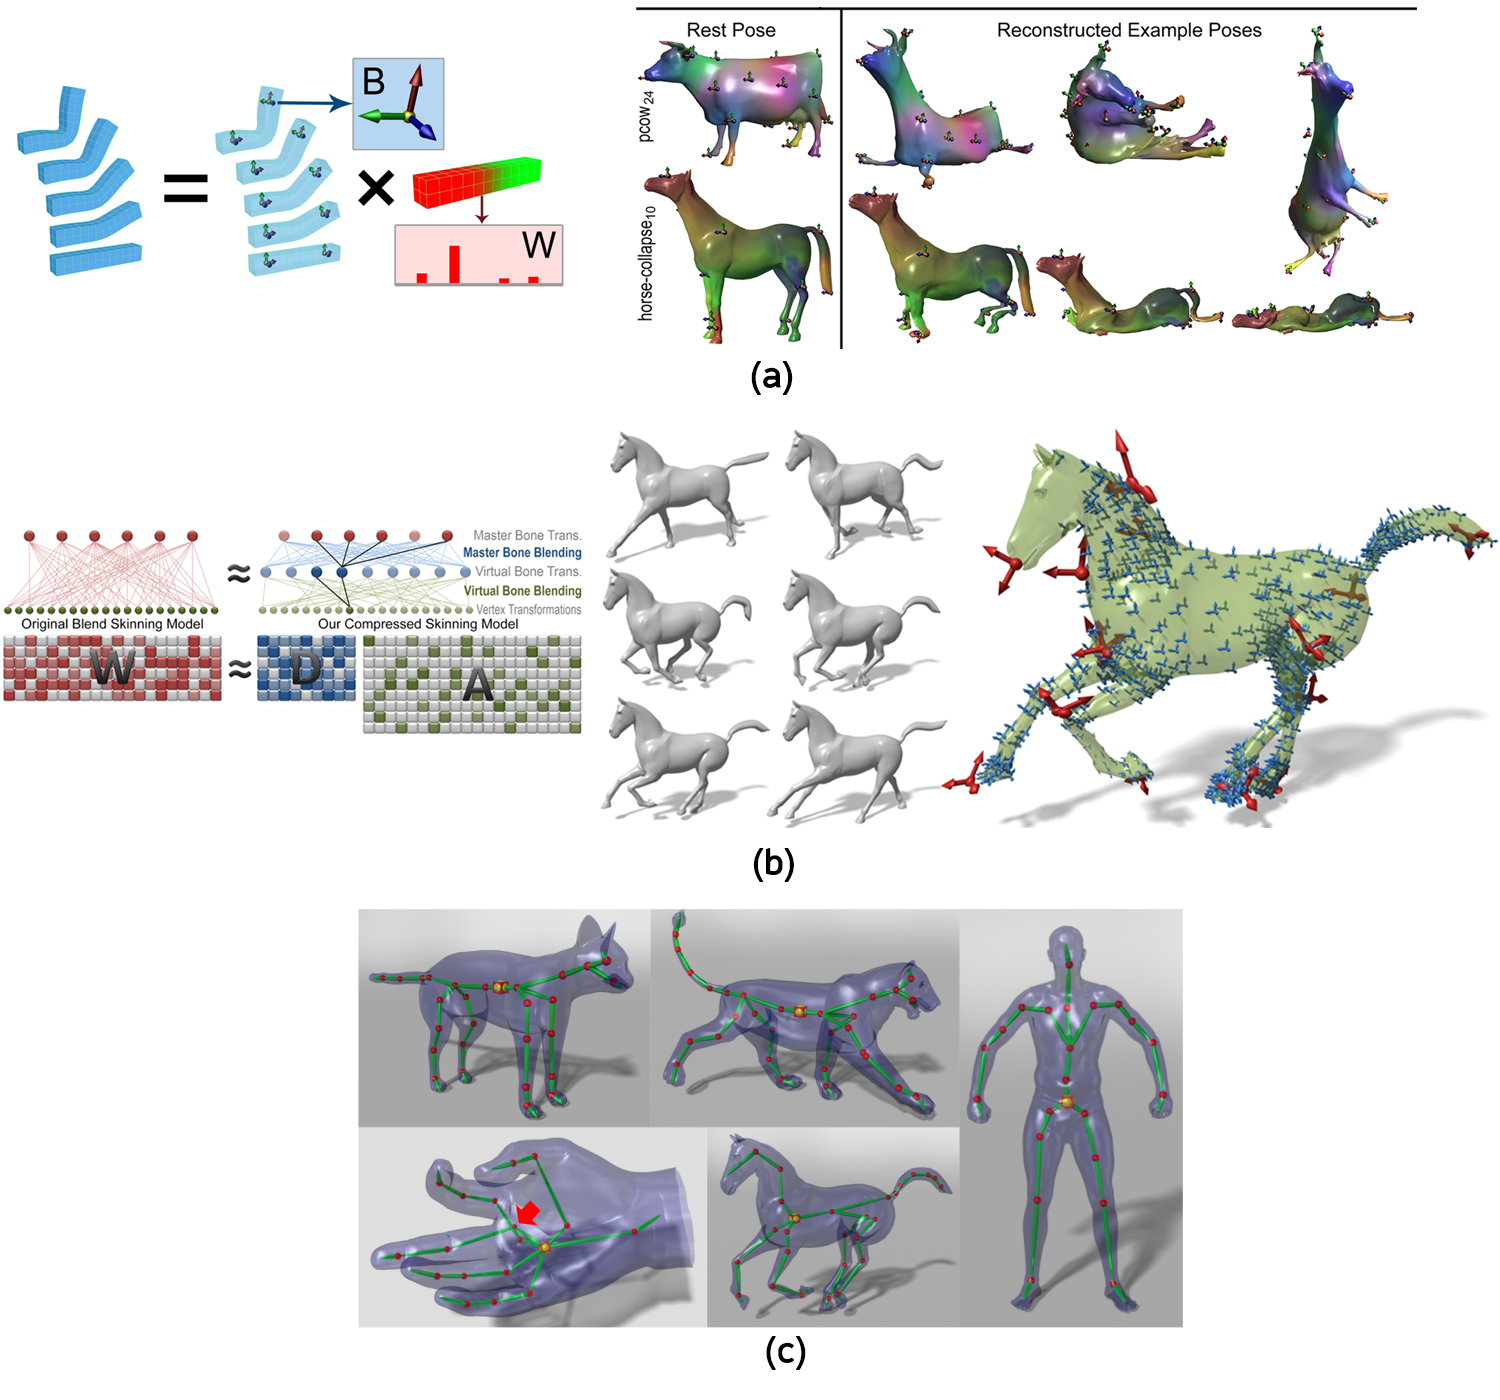
\includegraphics[width=3in]{images/skinning_decomposition}
  \caption{Sparse decomposition: skinning results. (a): \cite{le2012smooth}, left: a set of example poses are decomposed into rigid bone transformation B and a sparse, convex bone-vertex weight map W. right: results of SSDR on elastic models. (b): \cite{le2013two}, left: two-layer scheme. right: an animated mesh sequence and its corresponding compressed skinning model. (c): \cite{le2014ras}.}
\end{figure}


\subsection{Deformation}

Time-varying dynamic geometry with very fine dynamic shape detail can be generated and rendered at very high visual fidelity. When creating such content, artists usually rely on a low-dimensional control parameterization. Despite increasing expensive power of such parameterizations and simulations, producing such realistic animations from scratch is a labor-intensive process. Following the framework of  sparse PCA\cite{zou2006sparse,jenatton2011structured}, in order to decompose captured or animated mesh sequences into sparse, localized, and intuitive-to-control deformation component, \cite{neumann2013sparse} which propose a method that extracts sparse and spatially localized deformation modes from an animated mesh sequence by extending the theory of sparse matrix decompositions to 3D mesh sequence processing using $l_{1,1}$ norm as the sparse constraint(Figure).

\begin{figure}[ht]
  \centering
  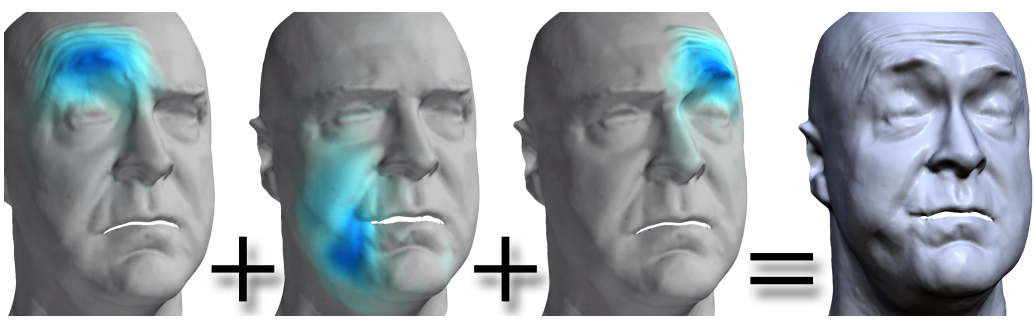
\includegraphics[width=3in]{images/localdefor_learning}
  \caption{Sparse decomposition: deformation\cite{neumann2013sparse}. A new facial expression is generated by summing deformation components.}
\end{figure}


Until now, we haven't given any discussion about the overcomplete dictionary $\mathbf{D}$ that exactly leads to the sparse representations of signals. From the definition of sparse representation, it is obvious that the choice of the dictionary will directly affect the signal processing result. In general, this dictionary can either be chosen as a prespecified set of functions(e.g., wavelet dictionary) or designed by adapting its content to fit a given set of signal examples(e.g., \cite{aharon2006svd}) which is preferred in most signal processing works. Here, we regard it as the sparse decomposition since the representation of a signal is the multiplication of a overcomplete dictionary, which is different from the former simple matrix, and its $sparse$ coefficient. Now that the dictionary could be learned from signals themselves, it could of course simply some processing objects such as point cloud to reduce the computational and memory cost. Compression is no doubt a good application.

\subsection{Compression}

The compression of unorganized point clouds have also attracted much attention due to the drastic improvement in scanner acquisition devices yielding point sets of tens of millions of points at high precision. But the counterpart of this development are datasets requiring ever higher storage capacity which results in the expensive cost in point cloud processing. \cite{digne2014self} uses the K-SVD algorithm \cite{aharon2006svd}, which seeks the adapting overcomplete dictionaries to achieve the best representation for each element in a training signal set, to encode the local descriptions of the selected seed points which are called self-similarity exploitation. This compression is done at the resolution of the scanner enabling improved control of the point cloud resolution and the input point clouds can be oriented or non-oriented. In addition, the approach also achieves a filtering of noise whose magnitude is smaller that the scanner precision. Figure shows the compression result.

\begin{figure}[ht]
  \centering
  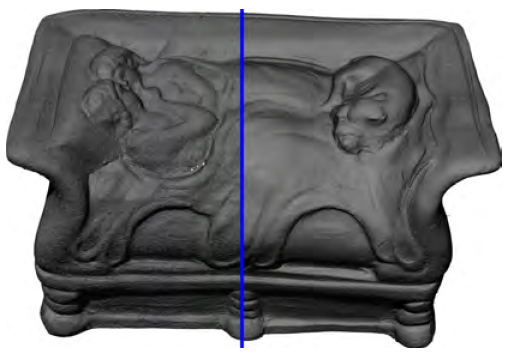
\includegraphics[width=3in]{images/compression_learning}
  \caption{Sparse decomposition: point cloud compression\cite{digne2014self}. The Lovers of Bordeaux(15.8 million points). Exploiting self-similarity in the model, they compress this representation down to 1.15 MB. The resulting model(right) is very close to the original one(left), as the reconstruction error is less than the laser scanner precision(0.02mm) for 99.14\% of the input points.}
\end{figure}

Last year, \cite{miandji2013learning} presents an algorithm for compression and real-time rendering of surface light fields(SLF) encoding the visual appearance of objects in static scenes with high frequency variations. After analyzing the spatial correlation in the data, they use a leaning based approach, Clustered Exemplar Orthogonal Bases(CEOB), to train a compact dictionary of orthogonal basis pairs, enabling efficient sparse projection of the SLF data. This method has an overall advantage in terms of memory footprint, rendering performance and reconstruction error.

\begin{figure}[ht]
  \centering
  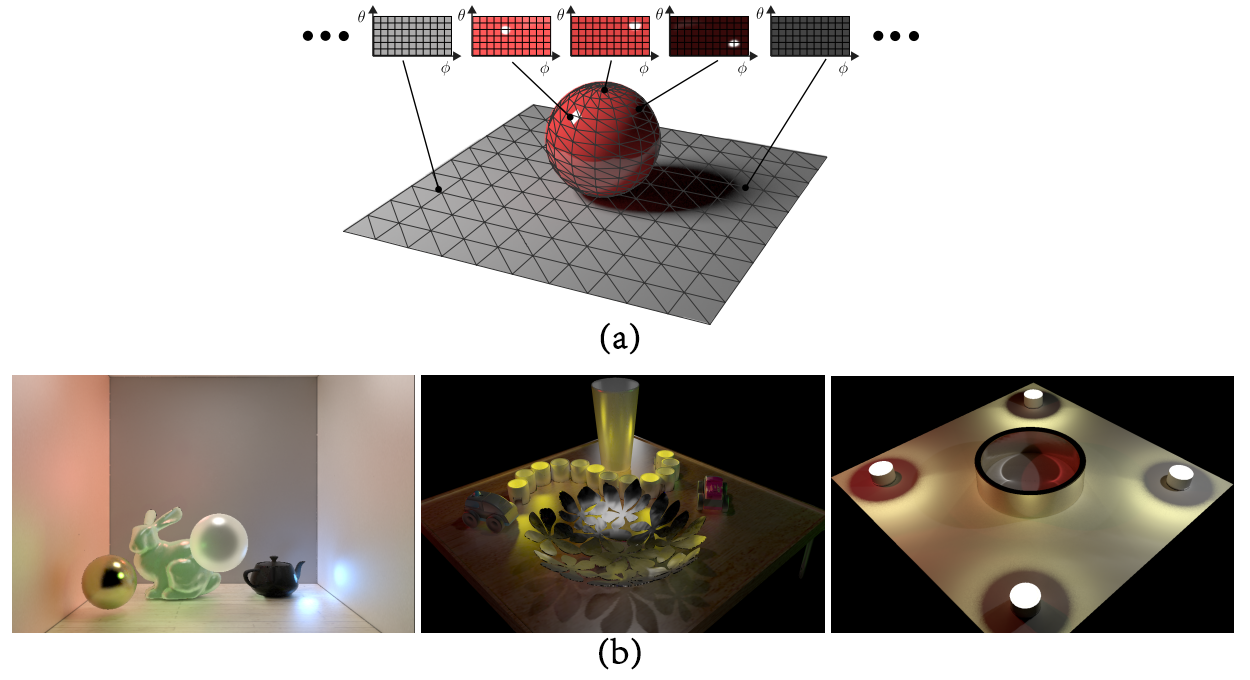
\includegraphics[width=3in]{images/rendering_learning}
  \caption{Sparse decomposition: rendering\cite{miandji2013learning} results using CEOB for three scenes with different materials.}
\end{figure}

\begin{figure}[ht]
  \centering
  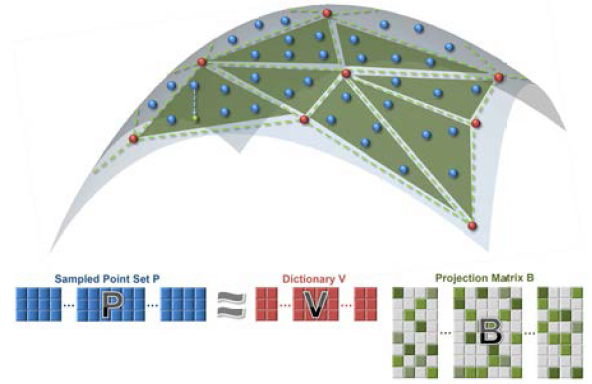
\includegraphics[width=3in]{images/reconstruction_learning}
  \caption{Sparse decomposition: reconstruction\cite{}. Left: an illustration of the reconstruction problem. Right: reconstruction of the Merlion model.}
\end{figure}



\subsection{Reconstruction}
